\documentclass[usenames,dvipsnames]{beamer}
% \documentclass[usenames,dvipsnames,handout]{beamer}

\usetheme{AnnArbor}
% \usecolortheme{default}
% \usecolortheme{crane}
\usecolortheme{beaver}
\usecolortheme{dolphin}
% \usecolortheme{orchid}
% \usecolortheme{rose}


\usepackage{fourier}
\usepackage{faktor}
\usepackage{amssymb}
\usepackage{amsmath}
\usepackage{amsthm}
%\usepackage{stmaryrd}
\usepackage{hyperref}
\usepackage[all]{xy}
\usepackage{tikz}
    \usetikzlibrary{mindmap,shadows,shapes.geometric,shapes.misc,positioning}
\usepackage{tikz-cd}
\tikzset{
    invisible/.style={opacity=0},
    visible on/.style={alt={#1{}{invisible}}},
    alt/.code args={<#1>#2#3}{%
      \alt<#1>{\pgfkeysalso{#2}}{\pgfkeysalso{#3}}%
  }
}
%\usetikzlibrary{matrix}
%\usetikzlibrary{calc,intersections}
%\newcommand{\downmapsto}{\rotatebox[origin=c]{-90}{$\large\mapsto$}\mkern2mu} %MnSymbol doesn't work well with beamer
\usepackage{multirow}

\def\Q{\mathbb{Q}}
\def\Z{\mathbb{Z}}
\def\C{\mathbb{C}}
\def\R{\mathbb{R}}
\def\F{\mathbb{F}}

\DeclareMathOperator{\AV}{AV}
\DeclareMathOperator{\Mat}{Mat}
\DeclareMathOperator{\Pol}{Pol}
\DeclareMathOperator{\Char}{char}
\DeclareMathOperator{\rk}{Rank}
\DeclareMathOperator{\Frob}{Frob}
\DeclareMathOperator{\ICM}{ICM}
\DeclareMathOperator{\Pic}{Pic}
\DeclareMathOperator{\Aut}{Aut}
\DeclareMathOperator{\Hom}{Hom}
\DeclareMathOperator{\End}{End}
\DeclareMathOperator{\Gal}{Gal}
\DeclareMathOperator{\mSpec}{mSpec}
\DeclareMathOperator{\GL}{GL}
\DeclareMathOperator{\Tr}{Tr}
\DeclareMathOperator{\Jac}{Jac}
%\renewcommand{\char}{char} %CRASHES WITH beamer


\newcommand{\cG}{\mathcal{G}}
%\newcommand{\cB}{{\mathcal B}}
\newcommand{\cA}{{\mathcal A}}
\newcommand{\cC}{{\mathcal C}}
\newcommand{\cO}{{\mathcal O}}
\newcommand{\cH}{{\mathcal H}}
%\newcommand{\cM}{{\mathcal M}}
\newcommand{\cT}{{\mathcal T}}
\newcommand{\cW}{{\mathcal W}}


\newcommand{\vphi}{\varphi}

\newcommand{\p}{{\mathfrak p}}
\newcommand{\frf}{{\mathfrak f}}

\newcommand{\downmapsto}{\rotatebox[origin=c]{-90}{$\large\mapsto$}\mkern2mu} %MnSymbol doesn't work well with beamer
\newcommand{\set}[1]{\left\lbrace#1\right\rbrace }
\newcommand{\Span}[1]{\left<#1\right>}

%\newcommand{\AVord}[1]{\AV^{\text{ord}}({#1})}
%\newcommand{\Modord}[1]{\cM^{\text{ord}}({#1})}

%\newcommand{\AVcs}[1]{\AV^{\text{cs}}({#1})}
%\newcommand{\Modcs}[1]{\cM^{\text{cs}}({#1})}

\newcommand{\Palpha}[2]{\mathcal{P}^{\alpha}_{{#1}}({#2})}
\newcommand{\Pone}[2]{\mathcal{P}^{1}_{{#1}}({#2})}

\newcommand{\red}[1]{\textcolor{red}{#1}}
\newcommand{\blue}[1]{\textcolor{blue}{#1}}
\newcommand{\green}[1]{\textcolor{ForestGreen}{#1}}

\newtheorem{df}{Definition}[section]
\newtheorem{remark}[df]{Remark}
\newtheorem{prop}[df]{Proposition}
\newtheorem{cor}[df]{Corollary}



%AUTHOR DETAILS
%%%%%%%%%%%%%%%%%%%%%%%%%%%%%%%%%%%%%%%%%%%%%%%%
\title[]{ Abelian varieties over finite fields\\ and their group of points }
\subtitle{}
\author[Stefano Marseglia]{Stefano Marseglia}
\institute[]{UPF - Gaati Lab}
\date[ 12/04/2024 ]{Géométrie et algèbre effectives - IRMAR - 12/04/2024}

\begin{document}

\begin{frame}
    \titlepage
\end{frame}

\begin{frame}{What do I do for a living?}
    \begin{center}
    \begin{tikzpicture}[
         % squarenodered/.style={rectangle, draw=red!60, fill=red!5, very thick, minimum size=5mm},
         % squarenodeblue/.style={rectangle, draw=blue!60, fill=blue!5, very thick, minimum size=5mm},
         squarenodepurple/.style={rectangle, draw=Black!60, fill=Black!5, very thick, minimum size=5mm},
         % CAlg/.style={rectangle},
         ]
         \onslide<1->{
              \begin{scope}[blend group=darken]
                   \filldraw[color=red!60, fill=red!30] (-2,0) ellipse (3cm and 2cm);
                   \filldraw[color=blue!60, fill=blue!30] (2,0) ellipse (3cm and 2cm);
                   \onslide<4->{\filldraw[color=Orange!60, fill=Yellow!30] (0,-2) ellipse (3cm and 2cm);}
              \end{scope}
              \node (AGset) at (-3,0)
                   {\parbox[c]{4em}{\Large Algebraic\\ Geometry}};
              \node (NTset) at (3,0)
                   {\parbox[c]{4em}{\Large Number\\ Theory}};
         }
         \onslide<4->{
              \node (CAlg) at (-0.5,-2.8)
                   {\parbox[c]{4em}{\centering \Large Commutative \\ Algebra}};   
         }
         \onslide<2->{
                \node[squarenodepurple] (AV) at (-0.5,2.8)    
                     {\parbox[c]{7.5em}{\centering Abelian Varieties: \\ add two points}};
                \draw [-,Black, very thick] (AV.south) .. controls (-0.5,1) ..  (0,0);
         }
         \onslide<3-4>{
                 \node[right=1cm of AV, anchor=west, yshift=-0.5cm] (Abel)
                            {\parbox{3.5cm}{\centering Niels Abel \footnotesize(1802-1829)\\
                                             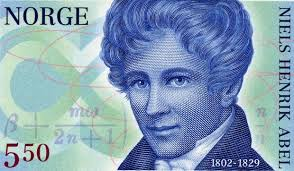
\includegraphics[width=3.5cm]{fig_abel.jpeg}
                            }};
                 \draw [dotted,black,very thick] (Abel) to [out=180,in=0] (AV);
         }
         \onslide<5->{
              \filldraw[color=Black!60, fill=Black!30] (0,0) circle (2cm);
              \node (Comp) at (-0.5,0)
                   {\parbox[c]{4em}{\centering \Large Computations \\ Algorithms}};
              }
         \end{tikzpicture}      
    \end{center}
\end{frame}

\begin{frame}{ Abelian varieties: what are they ? }
\vspace{-0.5cm}
\onslide<1->{Abelian varieties are connected projective group varieties.}
\begin{center}
   \begin{columns}
       \begin{column}{0.4\textwidth}
           \onslide<2->{Abelian varieties of dim.~$1$\\
                           are called {\bf elliptic curves}.\\
                           Eg: over $\R$, $\red{y^2 = x^3 -x +1}$
                           \vspace{1em}}
              % \vpsace{1em}
           \onslide<3->{We can add points:\\
                           $P,Q$ {\Large \blue{$\leadsto$}} $P\oplus Q$
                           \vspace{1em}\\
                           }
              \onslide<4->{Equations are impractical in $\dim \geq 2$.\\
                           We need a better way to represent them...}             
       \end{column}
       \begin{column}{0.5\textwidth}
           \tikz{
               \onslide<2->{
               \draw [help lines] (-2,-2.24) grid (1.8,2.24);
               \draw [->] (-2-0.2,0) -- (1.8+0.2,0) node[right] {$x$}; 
               \draw [->] (0,-2.24-0.2) -- (0,2.24+0.2) node[left] {$y$}; 
               \draw [red, thick, domain=-1.32471795724474602596090885448:1.8, samples=100]
                plot (\x, {sqrt(\x*\x*\x -\x +1)});
               \draw [red, thick, domain=-1.32471795724474602596090885448:1.8, samples=100]
                plot (\x, -{sqrt(\x*\x*\x -\x +1)});
               }
               \onslide<2->{
               \draw [blue, thick, domain=-2:1.8, samples=100] plot (\x, {0.7*\x +0.5 });
               \draw [blue, thick, dashed] (1.3407,2.24) -- (1.3407,-2.24);
               \draw (-1.2858-0.2,-0.7*1.2858+0.5+0.1) node {$P$};
               \draw (0.43506,0.7*0.43506+0.5 +0.3) node {$Q$};
               \draw (1.3407+0.5,-0.7*1.3407-0.5) node {$P\oplus Q$};
               }
           }
       \end{column}
   \end{columns}
\end{center}
\end{frame}

\begin{frame}{ Abelian varieties over $\C$ vs $\F_q$ }    
    \begin{itemize}
     \item Let $A/\C$ be an abelian variety of dimension $g$. 
\pause
    \item Then $A(\C)$ is a {\bf torus}: $T:=\C^g/\Lambda$, where $\Lambda\simeq_\Z\Z^{2g}$.
\pause 
    \item $T$ admits a non-degenerate Riemann form $\longleftrightarrow$ polarization.
\pause
    \item In fact, $ A \mapsto A(\C)$ induces an \blue{equivalence} of categories:
    \vspace{-.2cm}
	  \[
      \set{ \text{abelian varieties $/\C$} } \longleftrightarrow 
      \set{\parbox[c]{12.5em}{\center $\C^g/\Lambda$ with $\Lambda\simeq \Z^{2g}$ admitting\\ a Riemann form}}.
     \]
\pause
    \vspace{-.5cm}
    \item In \red{char.~$p>0$} such an equivalence \red{cannot exist} : there are (supersingular) elliptic curves with quaternionic endomorphism algebras.
\pause 
    \item Nevertheless, over finite fields, we obtain analogous results if we restrict ourselves to certain {\bf subcategories} of AVs...
\pause
    \item ... which we are going to use to \red{classify the AVs up to isomorphism}.
	\end{itemize}
\end{frame}

\begin{frame}{ Isogeny classification over $\F_q$}
	\begin{itemize}
    \item An {\bf isogeny} $A\to B$ is a surjective morphism with finite kernel.
\pause     
    \item $A/\F_{q}$ comes with a {\bf Frobenius} endomorphism, 
\pause
    that induces an action
		\[ \Frob_A : T_\ell A \rightarrow T_\ell A \text{ for any }\ell\neq p, \]
		where $T_\ell(A) = \varprojlim A[\ell^n] \simeq \Z_\ell^{2g}$.
\pause
    \item $\blue{h_A(x)}:=\Char(\Frob_A)$ is a \blue{$q$-Weil} polynomial and {\bf isogeny invariant}.
\pause
    \item By {\bf Honda-Tate} theory, the association
		\[ \text{isogeny class of }A \longmapsto h_A(x) \]
		is injective and allows us to \blue{enumerate} all AVs up to isogeny.
\pause
    \item Also, $h_A(x)$ is squarefree $\iff$ $\End(A)$ is commutative.
	\end{itemize}
\end{frame}

\begin{frame}{ Deligne's equivalence }
	Recall: $A/\F_q$ is {\bf ordinary} if half of the $p$-adic roots of $h_A$ are units.
\pause
	\begin{theorem}[Deligne '69]
	Let $q=p^r$, with $p$ a prime.
	There is an \blue{equivalence} of categories:
	\[ \begin{array}{cc}
	\set{\text{ {\bf Ordinary} abelian varieties over } \F_q } 	& A \\
\pause
    \updownarrow											& \downmapsto \\
	\set{\parbox[p]{19em}{pairs $(T,F)$, where $T\simeq_\Z \Z^{2g}$ and $T\overset{F}{\to} T$ s.t.\\
\pause
	- $F\otimes \Q$ is semisimple\\
	- the roots of $\Char_{F\otimes\Q}(x)$ have abs. value $\sqrt{q}$\\
	- \textbf{half of them are $p$-adic units}\\
	- $\exists V:T\to T$ such that $FV=VF=q$
	}}	& (T(A),F(A))
	\end{array} \]
	\end{theorem}
% \pause
% 	\begin{itemize}
% 	 \item Ordinary $A/\F_q$ can be canonically lifted: $\leadsto \cA_{\mathrm{can}}/\mathrm{Witt}(\F_q)$...
% \pause
% 	 \item ... characterized by: $\End_{\F_q}(A) = \End_W(\cA_{\mathrm{can}})$.
% \pause
% 	 \item Put $T(A):=H_1(\cA_{\mathrm{can}}\otimes \C,\Z) $
% \pause
% 	  and $F(A):=$ the induced Frobenius.
% 	\end{itemize}
\end{frame}

\begin{frame}{Squarefree case}
	\begin{itemize}
	\item Fix an \textbf{ordinary squarefree} $q$-Weil polynomial \blue{$h$} :
\onslide<2->  
    \item  $\rightsquigarrow \text{an isogeny class } \blue{\cC_h}$/$\F_q$.
\onslide<3->
    \item Put $K := \Q[x]/(h)=\Q[F]$, an \'etale algebra = product of number fields.
\onslide<4->
	\item Put $V=q/F$. Deligne's equivalence induces:
\onslide<5->
			\begin{theorem}
			\[\begin{array}{cc}
			\faktor{\set{\text{abelian varieties over $\F_q$ in $\cC_h$}}}{
\onslide<6->{\simeq}
            } & \\
			\updownarrow & \\
			\faktor{\set{ \text{fractional ideals of $\Z[F,V] \subset K$ } }}{
\onslide<6->{\simeq}
             } &
\onslide<7-> =:  \blue{\ICM(\Z[F,V])}\\ 
			& \blue{\text{ ideal class monoid} }
			  \end{array}\]
			\end{theorem}
\onslide<8->
    \item \red{Problem:} $\Z[F,V]$ might not be maximal $\rightsquigarrow $ \red{non-invertible} ideals.
	\end{itemize}
\end{frame}

\begin{frame}{ICM : Ideal Class Monoid}
    Let $R$ be an {\bf order} in an \'etale  $\Q$-algebra $K$.
% according to Bourbaki etale (over a field K) implies commutative and finite (since it is defined as being isomorphic to L^n for some extension L of K).
    \begin{itemize}
\pause
    \item Recall: for {\bf fractional $R$-ideals} $I$ and $J$
	 \[ I\simeq_R J \Longleftrightarrow \exists x \in K^\times \text{ s.t.~} xI=J \]
\pause
    \item We have
   	\begin{align*}
    \ICM(R) & \supseteq \Pic(R)=\faktor{\set{\text{invertible fractional $R$-ideals}}}{\simeq_R} \\
	\blue{\text{with equality }} & \blue{\rotatebox[origin=c]{90}{$\large\rightsquigarrow$}\mkern2mu \text{ iff } R=\cO_K }
    \end{align*}
\pause 
    \item ...and actually
    \[ \ICM(R) \supseteq \bigsqcup_{\scriptsize\parbox{5 em}{$R\subseteq S \subseteq \cO_K$\\over-orders}}\Pic(S) \qquad   
     \textcolor{blue}{\text{with equality iff $R$ is Bass}} \]
\pause
    \item Hofmann-Sircana '19: computation of over-orders.
\end{itemize}
\end{frame}

\begin{frame}{ simplify the problem  }
    Study the isomorphism problem locally: (Dade, Taussky, Zassenhaus '62)
    \begin{itemize}
\pause 
    \item  \textbf{weak equivalence}:
    \[I_{\p}\simeq_{R_{\p}} J_{\p} \text{ for every } {\p} \in \mSpec(R)\]
\pause
    \vspace{-6mm}\[\Updownarrow\]
    \[1\in (I:J)(J:I)\quad \textcolor{blue}{\text{easy to check!}}\]
\pause
    \item Let $\cW(R)$ be the set of weak eq.~classes...\\
\pause
    ...whose representatives can be found in
    \[\set{\text{sub-$R$-modules of $\faktor{\cO_K}{\frf_R}$ }} \quad \textcolor{blue}{\parbox{10 em}{finite! and most of the time not-too-big ...}}\]
    where $\frf_R=(R:\cO_K)$ is the conductor of $R$.
    \end{itemize}
\end{frame}

\begin{frame}{ Compute $\ICM(R)$ }
\pause 
    Partition w.r.t. the multiplicator ring:
    \begin{columns}
    \begin{column}{0.5\textwidth}
      \[ \cW(R) = \bigsqcup_{R\subseteq S \subseteq \cO_K} \cW_S(R)\]
      \[ \ICM(R) = \bigsqcup_{R\subseteq S \subseteq \cO_K} \ICM_S(R)\]
    \end{column}
\pause
    \begin{column}{0.5\textwidth}  %%<--- here
    \begin{center}
    \textcolor{blue}{\parbox{10em}{the ``pedix'' $-_S$ means ``only classes with multiplicator ring S''}} 
    \end{center}
    \end{column}
    \end{columns}
\pause
    \begin{theorem}[M.]
    For every over-order $S$ of $R$, $\Pic(S)$ acts \red{freely} on $\ICM_S(R)$ and
    \[ \cW_S(R) = \ICM_S(R) / \Pic(S) \]
\pause
    Repeat for every $R\subseteq S \subseteq \cO_K$:
    \[ \rightsquigarrow \ICM(R).\]
    \end{theorem}
\end{frame}


\begin{frame}{ To sum up: }
    \begin{itemize}
    \item To sum up:
\pause
    \item Given a {\bf ordinary squarefree} $q$-Weil polynomial $h$ ...
\pause
    \item ... $\leadsto$ algorithm to \blue{compute the isomorphism classes} of AVs in the isogeny class $\cC_h$.
\end{itemize}
\pause    
    \begin{remark}
        Let $\cC_h$ be a {\bf squarefree} isogeny classes over the {\bf prime field $\F_p$}.
        Building on work by Centeleghe-Stix, we get a bijection between the isomorphism classes of AVs in $\cC_h$ and the ideal class monoid of $\Z[F,V]$, as above.
        But the functor is completely different! (eg.~It is contravariant)
    \end{remark}
\end{frame}


\begin{frame}{Dual varieties and Polarizations }
    Howe described \textbf{dual} varieties and \textbf{polarizations} on Deligne modules.
\pause
    \begin{theorem}\
    Let $A\in \cC_h$ with $h$ ordinary and squarefree. If $A\leftrightarrow I$, then:
    \begin{itemize}
\pause
    \item $A^\vee \leftrightarrow \overline{I}^t:=\set{ \overline{x} \in K : \Tr(xI)\subseteq \Z}$.
\pause
    \item if $\mu$ is an isogeny $A\to A^\vee$ then $\mu \leftrightarrow \lambda\in K^\times$ with
    $\lambda I \subseteq \overline{I}^t$.
\pause
    \item $\mu$ is a polarization if and only if\\
    - $\lambda$ is \blue{totally imaginary} ($\overline \lambda = -\lambda$);\\
    - $\lambda$ is $\Phi$-positive, where $\Phi$ is a CM-type of $K$ satisfying the \blue{Shimura-Taniyama} formula.\\ 
\pause
    \item if $(A,\mu) \leftrightarrow (I,\lambda)$ is a princ.~polarized ab.~var.~and $S=(I:I)$ then
    \vspace{-0.7em}
    \[\set{\parbox[p]{9em}{non-isomorphic princ. polarizations of $A$}} \longleftrightarrow \dfrac{\set{\text{totally positive }u\in S^\times }}{\set{v\overline{v}: v\in S^\times}},\]
    \vspace{-1.5em}
\pause
    \item  and $\Aut(A,\mu) = \set{\text{torsion units of $S$}}$.
    \end{itemize}
    \end{theorem}
\end{frame}


\begin{frame}{Principal Polarizations}
    We have an {\bf algorithm} to enumerate principal polarizations up to isomorphism:
\pause
    \begin{enumerate}
    \item Compute $i_0$ such that $i_0 I = \overline{I}^t$.
\pause
    \item Loop over the representatives $u$ of the finite quotient
    \[ \frac{S^\times}{\set{v\overline{v}: v\in S^\times}}. \]
\pause    
    \item If $\lambda:=i_0 u$ is totally imaginary and $\Phi$-positive ...
\pause    
    \item ... then we have one principal polarization.
\pause    
    \item By the previous Theorem, we have all princ.~polarizations up to isom.
    \end{enumerate}
\pause 
    Can modify to compute polarizations of any degree.
\end{frame}

\begin{frame}{Example}
	\begin{itemize}
    \item Let $h(x)=x^8 - 5x^7 + 13x^6 - 25x^5 + 44x^4 - 75x^3 + 117x^2 - 135x + 81$, LMFDB label: 4.3.af\_n\_az\_bs.
\pause
    \item $\rightsquigarrow$ isogeny class of a simple ordinary abelian varieties over $\F_{3}$ of dimension $4$.
\pause
    \item Let $F$ be a root of $h(x)$ and put $R:=\Z[F,3/F]\subset \Q(F)$.
\pause
    \item $8$ over-orders of $R$: two of them are not Gorenstein.
\pause
    \item $\#\ICM(R) = 18 \rightsquigarrow 18$ isom.~classes of AV in the isogeny class.
\pause
    \item $5$ are not invertible in their multiplicator ring.
% \pause
%     \item $8$ classes admit principal polarizations.
% \pause
%     \item $10$ isomorphism classes of princ. polarized AV.
\pause
    \item More info at {\footnotesize \url{https://abvar.lmfdb.xyz/Variety/Abelian/Fq/4/3/af_n_az_bs}}
	\end{itemize}
\end{frame}


\begin{frame}{Example}{}
    Concretely:
	{\scriptsize \begin{align*}
	\begin{split} 
	I_1 = & 2645633792595191 \Z \oplus (F + 836920075614551) \Z \oplus (F^2 + 1474295643839839)\Z \oplus\\
	& \oplus (F^3 + 1372829830503387)\Z \oplus (F^4 + 1072904687510)\Z \oplus\\
	& \oplus \frac{1}{3}(F^5 + F^4 + F^3 + 2F^2 + 2F + 6704806986143610)\Z \oplus\\
	& \oplus \frac{1}{9}(F^6 + F^5 + F^4 + 8F^3 + 2F^2 + 2991665243621169) \Z \oplus\\
	& \oplus \frac{1}{27}(F^7 + F^6 + F^5 + 17F^4 + 20F^3 + 9F^2 + 68015312518722201)\Z\\
	\end{split}
	\intertext{principal polarizations:}
	\begin{split}
	x_{1,1} = \frac{1}{27}( & -121922F^7 + 588604F^6 - 1422437F^5 +\\
			  & +1464239F^4 + 1196576F^3 - 7570722F^2 + 15316479F - 12821193)\\ 
	%   \end{split}\\
	%   \begin{split}
	x_{1,2} = \frac{1}{27}( & 3015467F^7 - 17689816F^6 + 35965592F^5 -\\
			  & -64660346F^4 + 121230619F^3 - 191117052F^2 + 315021546F - 300025458)\\
	  \end{split}\\
	& \End(I_1) =  R\\
	& \#\Aut(I_1,x_{1,1}) = \#\Aut(I_1,x_{1,2}) = 2
	\end{align*}}
\end{frame}


\begin{frame}{ }
    \begin{itemize}
    \item The equivalence is not just useful to classify the AVs!
    \pause
    \item It can be used to compute polarizations, isogenies, and ...
    \pause
    \item ... group of $\F_q$-points.
    \pause
    \item In the rest of the talk, we will prove
    \end{itemize}
    \begin{theorem}[M.-Springer]
        Let $k$ be $\F_2$, $\F_3$ or $\F_5$. Let $G$ be a finite abelian group.
        \pause
        Then there exists an ordinary $A/k$ with $A(k) = G$.
    \end{theorem}
\end{frame}


\begin{frame}{ Cyclic abelian varieties }\
    Recall that we have an equivalence
    \[ \cC_h \longleftrightarrow \set{\text{fractional ideals of $\Z[F,q/F]$}}. \]
    \pause
    \vspace{-0.5cm}
    \begin{corollary}
        If $A$ corresponds to the fractional $\Z[F,q/F]$-ideal $J$ then
    \pause
        \vspace{-0.2cm}
        \[ A(\F_q) \simeq \frac{J}{(1-F)J}.\]
    \end{corollary}
    \pause
    \begin{prop}[M.-Springer]
        Every ordinary squarefree isogeny class contains a cyclic abelian variety.
    \end{prop}
    \pause
	Proof: Take $A\longleftrightarrow J=\Z[F,q/F]$.
    \pause
    \[ A(\F_q)\simeq \frac{\Z[F,q/F]}{(1-F)} \simeq \frac{\Z[x,y]}{(h(x),xy-q,1-x)}
    \pause
    \simeq \frac{\Z}{h(1)\Z}.\qed \]
\end{frame}

\begin{frame}{ Number of points }
    \begin{theorem}[Howe-Kedlaya]
        Let $m\in\Z_{> 0}$. Then there is a squarefree ordinary $A/\F_2$ such that $\#A(\F_2)=m$.
    \end{theorem}
    \pause
    \begin{theorem}[van Bommel-Costa-Li-Poonen-Smith]
        Let $m\in\Z_{> 0}$ and $k$ be $\F_3$ or $\F_5$. Then there is a squarefree ordinary $A/k$ such that $\#A(k)=m$.
    \end{theorem}
    \pause
    They use extremely clever constructions that allows them to construct characteristic polynomials $h_A$ such that $h_A(1)=m$.
\end{frame}

\begin{frame}{ Group of points }
    \begin{theorem}[M.-Springer]
        Let $k$ be $\F_2$, $\F_3$ or $\F_5$. Let $G$ be a finite abelian group.
        \pause
        Then there exists an ordinary $A/k$ with $A(k) = G$.
    \end{theorem}
    \pause
    Proof: Write
    \[ G\simeq \frac{\Z}{m_1 \Z} \times \ldots \times \frac{\Z}{m_s \Z}.\]
    \pause
    By H-K or vBCLPS, for each $i$ there is an isogeny class with $m_i$ points.\\
    \pause
    By Proposition, within each of the isogeny classes, there is a cyclic $A_i$.\\
    \pause
    Take $A=\prod_i A_i$. \qed
    \pause
    \begin{corollary}
        If $G$ is cyclic we can take $A$ to be ordinary and squarefree.
    \end{corollary}
\end{frame}

\begin{frame}{ Further results (building on vBCLPS) }
	\begin{itemize}
        \pause
        \item Over $\F_4$: for every abelian $G$ there exists an ordinary or almost ordinary $A/\F_4$ such that $A(\F_4)\simeq G$.
        \pause
        \item Over $\F_7$: for every cyclic $G$ with $\# G\not \in \set{2,8,14,16,17,73}$ there exists a squarefree ordinary $A/\F_7$ such that $A(\F_7)\simeq G$.
        \pause
        \item vBCLPS: For an arbitrary $q$, every integer $m\geq q^{3\sqrt{q}\log q}$ arises as $m=\#A(\F_q)$ for some ordinary squarefree $A/\F_q$.
	\end{itemize}
    \pause
    \begin{theorem}[M.-Springer]
        Let $m_1,\ldots,m_r$ be integers satisfying $m_i\geq q^{3\sqrt{q}\log q}$.
        Put
        \[ G=\frac{\Z}{m_1 \Z}\times \ldots \times \frac{\Z}{m_r \Z}. \]
        \pause
        Then there is an ordinary $A/\F_q$ such that $G=A(\F_q)$.
    \end{theorem}
\end{frame}

\begin{frame}{ }
    \begin{center}
        \green{\huge Thank you!}
    \end{center}
\end{frame}

\end{document}
